% ------------------------------------------------------------------
%  Section: the zero-point flux of the mode moves the 0-pi boundary (data/nonadiabatic, fig_cavity_0pi)
% ------------------------------------------------------------------
\paragraph*{Flux-driven $0$--$\pi$ switch.}
Figure~\ref{fig:cavity0pi} contains the first result. Without the mode the junction is a $0$ junction for
$U<U_c^0=0.94\Delta$, where the singlet is the ground state at zero flux, and a $\pi$ junction above (SM).
With the mode we compute the ground state of Eq.~\eqref{eq:H} in both parity sectors at $\varphi_{\rm cl}=0$,
without any seed, for $\hbar\omega=0.01$--$3\,\Delta$ and $g\le1$, and locate the boundary $U_c(g,\omega)$ of
the \emph{loop} from the crossing $E_{\rm odd}=E_{\rm even}$. At $U=0.9\Delta$ and $\hbar\omega=0.1\Delta$
[Fig.~\ref{fig:cavity0pi}(a)] the doublet--singlet energy difference falls from $+0.010\Delta$ at $g=0$ to
$-0.008\Delta$ at $g=0.4$ and $-0.065\Delta$ at $g=1$: the loop switches from $0$ to $\pi$ at $g\simeq0.28$,
a mode impedance $Z\simeq0.6\,{\rm k}\Omega$, with nothing but the vacuum of the mode acting on the junction.
The boundary $U_c(g,\omega)$ [Fig.~\ref{fig:cavity0pi}(b)] moves down at every $\omega$: to $0.83\Delta$ at
$g=0.5$ and to $0.65$, $0.60$ and $0.57\Delta$ at $g=1$ for $\hbar\omega=0.1$, $0.3$ and $1\,\Delta$, i.e.\ by
$30$--$40\%$ of $U_c^0$.

The mechanism changes with $\hbar\omega$. For $\hbar\omega\ll E_A$ the exact boundary coincides with that of
the circuit model~\eqref{eq:BO} (dashed; $0.889$ against $0.889\Delta$ at $g=0.4$ and $0.813$ against
$0.815\Delta$ at $g=0.8$ for $\hbar\omega=0.01\Delta$): the zero-point motion of the flux samples $E_s(gX)$
around $\varphi=0$, where the singlet surface curves up ($E''_{\rm even}(0)=+0.20\Delta$) and the doublet
surface curves down, so that the singlet loses and the doublet gains zero-point energy,
$\delta E_s\simeq\tfrac12g^2E''_s(0)\langle X^2\rangle$, and for $gX$ of order one the doublet lowers its
energy further by letting the flux relax towards $\Phi_0/2$, where its minimum lies. This is the quantum
version of the parity switch by a free flux discussed below. As $\hbar\omega$ grows the exact boundary
leaves the circuit model (by $0.015$, $0.032$ and $0.040\Delta$ at $g=0.8$ for $\hbar\omega=0.1$, $0.3$ and
$1\,\Delta$) and settles on the Lang--Firsov line (dotted) at $\hbar\omega\simeq\Delta$: $0.663$ against
$0.670\Delta$ at $g=0.8$, and $\hbar\omega=3\Delta$ gives the same boundary to $10^{-3}\Delta$. There the mode no
longer follows the junction but reduces the level width of the dressed bond by $e^{-g^2}$, and the singlet,
which is bound by $\Gamma$, loses against the doublet. The adiabatic shift is bounded by the condensation
energy of the $\pi$ well, the Franck--Condon shift by $\Gamma$ alone, and the corrections $O(t_J^2/\hbar\omega)$
are below $0.01\Delta$ at $\hbar\omega=\Delta$. The dressing of the
junction is visible in the Peierls factor and in the photon--electron entanglement
[Fig.~\ref{fig:cavity0pi}(c)]: $|\langle D\rangle|$ follows $e^{-g^2/2}$ for $\hbar\omega\gtrsim0.3\Delta$,
where the mode is only squeezed by its vacuum, and falls faster in the adiabatic regime, where it is
displaced towards the $\pi$ well; the entanglement entropy is largest there ($0.26$ at $g=0.8$,
$\hbar\omega=0.01\Delta$), because the flux state depends on the electronic sector.

The effect is not an artefact of the one-bond vertex: the neglected capacitive terms are of relative order
$\hbar\omega g^2/E_A$, and the shift of $U_c$ at $\hbar\omega=0.01\Delta$, where they are negligible, is
already half of the one at $\hbar\omega=0.3\Delta$. Nor is it a mean-field effect: the Hartree--Fock product
state replaces the Kramers doublet by a static moment and places the boundary at $0.82\Delta$ for every $g$
(next section). The prediction is that a dot junction gate tuned close to its singlet--doublet boundary, in a loop
whose inductance is a superinductor of impedance $Z\gtrsim1\,{\rm k}\Omega$, is driven into the $\pi$ phase
by the impedance alone, with the switch visible as the jump of the resonator frequency that marks the parity
transition in Refs.~\cite{Bargerbos2022,PitaVidal2023}.

\begin{figure*}
  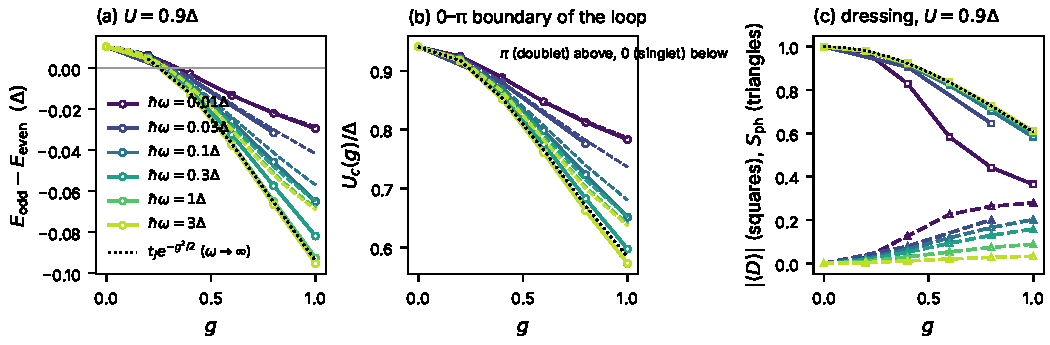
\includegraphics[width=\textwidth]{../figs/fig_cavity_0pi.pdf}
  \caption{\label{fig:cavity0pi}%
  Zero-point flux and the $0$--$\pi$ transition ($L=10$, $t_J=0.5\Delta$, $\varphi_{\rm cl}=0$, no seed).
  (a) Doublet--singlet energy difference versus $g$ at $U=0.9\Delta$ for $\hbar\omega=0.01$--$3\,\Delta$: full
  DMRG (symbols), circuit model~\eqref{eq:BO} with the $g=0$ surfaces (dashed), Lang--Firsov ring with
  $t_Je^{-g^2/2}$ on the dressed bond (dotted, the $\omega\to\infty$ limit). The sign change is the switch of the loop from $0$ to $\pi$.
  (b) Boundary $U_c(g,\omega)$ of the loop from the crossing $E_{\rm odd}=E_{\rm even}$ (same symbols and lines).
  (c) Dressing of the junction in the doublet sector at $U=0.9\Delta$: $|\langle D\rangle|$ (squares; dotted:
  $e^{-g^2/2}$) and the photon--electron entanglement entropy $S_{\rm ph}$ (triangles).}
\end{figure*}
